%\VignetteEngine{knitr::knitr}
%\VignetteIndexEntry{Imputation Methods in robCompositions}
\documentclass{scrartcl}\usepackage[]{graphicx}\usepackage[]{color}
%% maxwidth is the original width if it is less than linewidth
%% otherwise use linewidth (to make sure the graphics do not exceed the margin)
\makeatletter
\def\maxwidth{ %
  \ifdim\Gin@nat@width>\linewidth
    \linewidth
  \else
    \Gin@nat@width
  \fi
}
\makeatother

\definecolor{fgcolor}{rgb}{0.345, 0.345, 0.345}
\newcommand{\hlnum}[1]{\textcolor[rgb]{0.686,0.059,0.569}{#1}}%
\newcommand{\hlstr}[1]{\textcolor[rgb]{0.192,0.494,0.8}{#1}}%
\newcommand{\hlcom}[1]{\textcolor[rgb]{0.678,0.584,0.686}{\textit{#1}}}%
\newcommand{\hlopt}[1]{\textcolor[rgb]{0,0,0}{#1}}%
\newcommand{\hlstd}[1]{\textcolor[rgb]{0.345,0.345,0.345}{#1}}%
\newcommand{\hlkwa}[1]{\textcolor[rgb]{0.161,0.373,0.58}{\textbf{#1}}}%
\newcommand{\hlkwb}[1]{\textcolor[rgb]{0.69,0.353,0.396}{#1}}%
\newcommand{\hlkwc}[1]{\textcolor[rgb]{0.333,0.667,0.333}{#1}}%
\newcommand{\hlkwd}[1]{\textcolor[rgb]{0.737,0.353,0.396}{\textbf{#1}}}%
\let\hlipl\hlkwb

\usepackage{framed}
\makeatletter
\newenvironment{kframe}{%
 \def\at@end@of@kframe{}%
 \ifinner\ifhmode%
  \def\at@end@of@kframe{\end{minipage}}%
  \begin{minipage}{\columnwidth}%
 \fi\fi%
 \def\FrameCommand##1{\hskip\@totalleftmargin \hskip-\fboxsep
 \colorbox{shadecolor}{##1}\hskip-\fboxsep
     % There is no \\@totalrightmargin, so:
     \hskip-\linewidth \hskip-\@totalleftmargin \hskip\columnwidth}%
 \MakeFramed {\advance\hsize-\width
   \@totalleftmargin\z@ \linewidth\hsize
   \@setminipage}}%
 {\par\unskip\endMakeFramed%
 \at@end@of@kframe}
\makeatother

\definecolor{shadecolor}{rgb}{.97, .97, .97}
\definecolor{messagecolor}{rgb}{0, 0, 0}
\definecolor{warningcolor}{rgb}{1, 0, 1}
\definecolor{errorcolor}{rgb}{1, 0, 0}
\newenvironment{knitrout}{}{} % an empty environment to be redefined in TeX

\usepackage{alltt}
\usepackage[pdftex]{hyperref}
\usepackage{amssymb, amsfonts}
%\usepackage[authoryear]{cite}
\usepackage[authoryear]{natbib}
%\usepackage{amsmath, amsfonts, amssymb} 
%\usepackage[authoryear]{natbib}
%\usepackage{graphicx,fancyhdr,vmargin}
%\usepackage{natbib}

\hypersetup{colorlinks,
        citecolor=blue,
        linkcolor=blue,
        urlcolor=blue
}

\def\R{\hbox{\znaky R}}
\def\A{\hbox{\znaky A}} \def\hA{\hbox{\hznaky A}}
\def\M{\hbox{\znaky M}}
\def\N{\hbox{\znaky N}}
\newcommand{\plural}[1]{\ensuremath{\underline{\mathbf{#1}}}}
\def\tucne#1{\mbox{\mathversion{bold}$#1$}}
\newcommand{\m}[1]{\ensuremath{\mathbf{#1}}}
%\renewcommand{\boma}[1]{\mbox{\boldmath ${#1}$}}
  
\newcommand{\Rlogo}{\raisebox{-.1mm}{
\includegraphics[width=1.2em]{logo.pdf}}}
\IfFileExists{upquote.sty}{\usepackage{upquote}}{}
\begin{document}



\begin{flushleft}
  {\LARGE\textbf{Robust Imputation of Missing
  Values in} \\[2mm]  \vspace*{-0.8cm} \textbf{Compositional Data Using the\Rlogo-Package} 
  \vspace*{0.55cm} \texttt{robCompositions}}
  \vspace{1.0cm}
  
  Matthias Templ$^{*,**}$, Peter Filzmoser$^{*}$, Karel Hron$^{***}$
  
{\small
\begin{description}
\item $^{*}\;$  Department of Statistics and Probability Theory, Vienna
University of Technology, Wiedner Hauptstr. 8-10, 1040 Vienna, Austria.
(\href{templ@tuwien.ac.at}{templ@tuwien.ac.at}) \\
\item $^{**}\;$    Department of Methodology, Statistics Austria, Guglgasse 13,
1110 Vienna, Austria.
(\href{matthias.templ@statistik.gv.at}{matthias.templ@statistik.gv.at}) and \\
\item $^{***}\;$ Department of Mathematical Analysis and Applications of
Mathematics, Palack\'y University, Tomkova 40, 779 00 Olomouc, Czech Republic. 
  (\href{hronk@seznan.cz}{hronk@seznan.cz})
\end{description}
}
\end{flushleft}
\vspace{1cm}



\begin{center} {\large Abstract} \end{center}

\abstract{The aim of this contribution is to show how the R-package
\texttt{robCompositions} can be applied to estimate missing values in
compositional data. Two procedures are summarized, one of them being
highly stable also in presence of outlying observations.
Measures for information loss are presented, and it is demonstrated
how they can be applied. Moreover, we introduce new diagnostic tools
that are useful for inspecting the quality of the imputed data.}


%%%%%%%%%%%%%%%%%%%%%%%%%%%%%%%%%%%%%%%%%%%%%%
\section{Introduction}


\subsection{Imputation}
Many different methods for imputation have been developed over the last few decades.
The techniques for imputation can be subdivided into four categories: univariate methods 
such as column-wise (conditional) mean or median imputation, distance-based imputation 
methods such as $k$-nearest neighbor imputation, covariance-based methods such as the 
well-known expectation maximization imputation method, and model-based methods such as 
regression imputation. 
%If an algorithm includes a certain kind of randomness it may be 
%adapted for multiple imputation.
Most of these methods are able to deal with missing completely at random (MCAR) 
and missing at random (MAR) missing values mechanism (see, e.g.
\cite{Little87}). However, most of the existing methods assume that the data originate 
from a multivariate normal distribution. 
This assumption becomes invalid as soon as there are outliers in the data. In that case
imputation methods based on robust estimates should be used.


\subsection{Compositional Data}

Advanced (robust) imputation methods have turned out to work well for data
with a direct representation in the Euclidean space. However, this is not 
the case when dealing with compositional data.

An observation
$\m{x}=(x_1,\dots,x_D)$ is called a $D$-part composition
if, and only if, all its components are strictly positive real numbers and all
the relevant information is included in the ratios between them
\citep{Aitchison86}.
One can thus define the \textit{simplex}, which is the sample space of $D$-part
compositions, as 
\begin{equation}
\mathcal{S}^D=\{\m{x}=(x_1,\dots,x_D),\,x_i> 0,\,\sum_{i=1}^Dx_i=\kappa\} \ \ .
\end{equation}
Note that the constant sum constraint $\kappa$ implies that $D$-part
compositions are only $D-1$ dimensional, so they are singular by definition.
It is, however, possible that the constant $\kappa$ is different for
each observation (for further details, see \cite{Hron09}). 
In any case, the important property of compositional data is that all information is 
contained in the ratios of the parts.

The application of standard statistical methods, like correlation analysis or principal 
component analysis, directly to compositional data can lead to biased and meaningless 
results \citep{Filzmoser08a, Filzmoser08b}. This is also
true for imputation methods \citep{bren08, Fern03, Boogaart06}.
A way out is to first transform the data with appropriate transformation methods.
Such transformations, preserving the specific geometry of compositional data on
the simplex (also called Aitchison geometry), are represented by the family of log-ratio
transformations: additive, centered \citep{Aitchison86} and isometric
(abbreviated by \textit{ilr}, \citep{Egozcue03} transformations.
Standard statistical methods can then be applied to the transformed data, and
the results can be back-transformed.

Compositional data frequently occur in official statistics. Examples are expenditure 
data, income components in tax data, wage components in the Earnings Structure Survey, 
components of turnover of enterprises etc., and all data which sum up to a
constant or which carry all the information only in the ratios.
The problem of missing values in compositional data including outliers is a common
problem not only in official statistics, but also in various other fields 
(see, e.g., \citep{Graf06, Filzmoser08a}).
In the following Section we will briefly review two algorithms for imputation
that are described in detail in \cite{Hron09}. Section 3 focuses on the 
use of the R-package \texttt{robCompositions}, and Section 4 introduces
some diagnostic tools implemented in this package. The final Section 5 concludes.


\section{Proposed Imputation Algorithms}

In the following we briefly describe the imputation methods that have been 
implemented in the R-package \texttt{robCompositions}. The 
detailed description of the algorithms can be found in \cite{Hron09}. 

\subsection{$k$-Nearest Neighbor Imputation}

$k$-nearest neighbor imputation usually uses the Euclidean distance
measure. Since compositional data are represented only in the simplex sample
space, we have to use a different distance measure, like the 
Aitchison distance, being
defined for two compositions $\m{x}=(x_1,\dots,x_D)$ and $\m{y}=(y_1,\dots,y_D)$ as
\begin{equation}
\label{adist}
d_a(\m{x},\m{y})=\sqrt{\frac{1}{D}\sum_{i=1}^{D-1}\sum_{j=i+1}^D
\left(\ln\frac{x_i}{x_j}-\ln\frac{y_i}{y_j}\right)^2} .
\end{equation}  
Thus, the Aitchison distance takes care of the property that compositional data
include their information only in the ratios between the parts.

Once the $k$-nearest neighbors to an observation with missing parts have been
identified, their information is used to estimate the missings. For reasons
of robustness, the estimation is based on using medians rather than means.
If the compositional
data do not sum up to a constant, it is important to use an adjustment according
the sum of all parts prior to imputation. For details, see \cite{Hron09}.


\subsection{Iterative Model-Based Imputation}

In the second approach we initialize the missing values with the proposed $k$-nearest 
neighbor approach. Then the data are transformed to the
$D-1$ dimensional real space using the ilr transformation.
Let $d_e$ denote the Euclidean distance. The ilr transformation holds the
so-called isometric property,
\begin{equation}
d_a(\m{x},\m{y})=d_e(ilr(\m{x}),ilr(\m{y})) 
\end{equation}
\citep{Egozcue05}. Consequently, one can use standard statistical methods 
like multiple linear regression, that work correctly in the Euclidean space.

We take a special form of the ilr transformation, namely
$ilr(\m{x})=(z_1,\dots,z_{D-1})$, with 
\begin{equation}
z_i=\sqrt{\frac{D-i}{D-i+1}}\,\ln\frac{\sqrt[D-i]{\prod_{j=i+1}^Dx_j}}{x_{i}}
\quad \mbox{ for } i=1,\ldots ,D-1 \ \ .
\end{equation}
Here, the compositional part $x_1$ includes the highest amount of missings,
$x_2$ the next highest, and so on. Thus, when performing a regression of 
$z_1$ on $z_2,\dots, z_{D-1}$, only $z_1$ will be influenced by the initialized
missings in $x_1$, but not the remaining ilr variables.

The idea of the procedure is thus to iteratively improve the estimation of the
missing values. After the regression of $z_1$ on $z_2,\dots, z_{D-1}$, the
results are back-transformed to the simplex, and the cells that were originally missing 
are updated. 
Next we consider the variable which originally has the second highest amount
of missings, and the same regression procedure as before is applied in the
ilr space. After each variable containing missings has been proceeded,
one can start the whole process again until
the estimated missings stabilize.
The detailed description of this algorithm can be found in \cite{Hron09}.

As a regression method we propose to use robust regression, like LTS regression
(see \cite{Maronna06}), especially if outliers might be present in the data.


\section{Using the R-package \texttt{robCompositions} for Imputing Missing Values}

%\subsection{Data Sets in the Package}
%
%Three data sets are included in the package, namely

%<<data sets>>=
%library(robCompositions)
%data(aitchison359)
%data(aitchison360)
%data(aitchison395)
%@
%
%These data sets can be found in the book from \cite{Aitchison86} on page 359,
%360 and 395.
%
%In the following we will use the aitchison395 data set which consists
%of household expenditures on five commodity groups of 20 single men. The
%variables represent housing (including fuel and light), foodstuff, alcohol and tobacco, 
%other goods (including clothing, footwear and durable goods) and services 
%(including transport and vehicles). Thus they represent
%the ratios of the men's income spent on the mentioned expenditures.
%
%For further proceeding we set some values to missing which then will be imputed
%with our proposed methods.
%
%<<aitchison395>>=
%x <- aitchison395
%x[1,3] <- x[2,4] <- x[3,3] <- x[3,4] <- NA
%@

\subsection{Data}

The package includes the three compositional data sets \textit{aitchison359},
\textit{aitchison360}, and \textit{aitchison395}, that have been published
in \cite{Aitchison86}. In the following, however, we will use simulated data,
where the data structure and outliers are exactly known.
The data generation is the same as described in \cite{Hron09}, and
a plot of the data set in shown in Figure \ref{repFig1} for the original
data (left) and for the ilr transformed data (right): We took 90 
observations with 3 parts that are normally distributed on the simplex
(i.e. they are multivariate normally distributed in the 2-dimensional
ilr space). A group of 5 outliers (\textit{group 1}) 
is added (green crosses in Figure \ref{repFig1})
that are potential outliers in the Aitchison and in the Euclidean space.
Another group (\textit{group 2}) of 5 outliers (blue triangles in Figure \ref{repFig1})
is only affecting the Euclidean space. Note that both types of outliers are
simulated to have a considerably higher sum of their parts, which is not visible
in the ternary diagram \citep{Aitchison86} in Figure \ref{repFig1} (left) where the parts
are re-scaled to have sum 1.

The generated (complete) data are stored in the list element \texttt{z2}
of object $x$. Among the non-outliers we set 20\% of the values in the first
part, 10\% in the second, and 5\% in the third part to missing, using an
MCAR mechanism. The new data set is stored in the list element \texttt{zmiss} of object $x$.

%% original:


%% neu:

 







\setkeys{Gin}{width=0.9\textwidth}
\begin{figure}[h]
\begin{center}
\vspace*{-3cm}
%<<plot-acomp, fig=TRUE, echo=FALSE>>=
%par(mfrow=c(1,2), mar=c(3.5,0,0,0))
%plot.acomp(acomp(x$z2), col=c(rep(1,90), rep(4,5), rep(3,5)), pch=c(rep(20,90), rep(2,5), rep(4,5)), cex=c(rep(0.6,90), rep(0.9,5), rep(0.9,5)))
%par(mar=c(3.5,4,0,0.1))
%plot(ilr(x$z2), col=c(rep(1,90), rep(4,5), rep(3,5)), pch=c(rep(20,90),
%rep(2,5), rep(4,5)), xlab=expression(z[1]), ylab=expression(z[2]), cex.lab=1.5, cex=c(rep(0.6,90), rep(0.9,5), rep(0.9,5))) 
%@
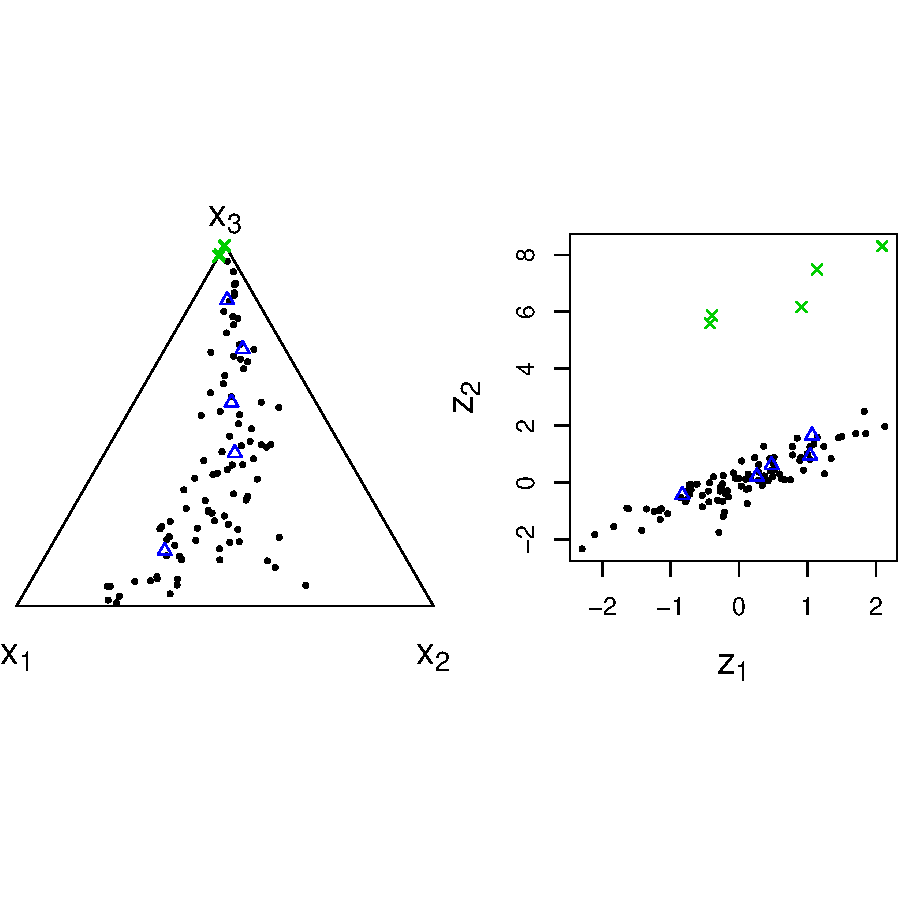
\includegraphics{plot-acomp}  
\vspace*{-33mm}
\caption{Simulated data set with 5 points from
\textit{outlier group 1} (symbol \textcolor{green}{$\times$}) 
and 5 points from \textit{outlier group 2} 
(symbol \textcolor{blue}{$\triangle$}).
Left plot: 3-part compositions shown in the ternary diagram;
right plot: data after ilr transformation.}
\label{repFig1}
\end{center}
\end{figure}



\subsection{Usage of the Imputation Methods Within the Package}


%A choice of methods is applied within the following lines of code:

%% real data set example:
%<<Imputation>>=
%xi1 <- impKNNa(x, k=4, metric="Aitchison")
%xi2 <- impKNNa(x, k=4, agg = "mean")
%xi3 <- impCoda(x, method="ltsReg", eps=0.01)
%xi4 <- impCoda(x, method="lm")
%xi5 <- impCoda(x, method="classical")
%@
%
%So, $k$-nearest neighbor imputation was performed (with aggregating
%the $k$-nearest neighbors for impuation with the median (\texttt{xi1}) and with
%the mean (\texttt{xi2}).
%In addition to that, our proposed iterative algorithms performed out,
%``ltsReg'' for robust iterative model based imputation (\texttt{xi3}), ``lm''
%for iterative model based imputation using least squares regressions
%(\texttt{xi4}), and by applying principal component analysis in an iterative
%way (\texttt{xi5}).
%
%Note that various other choices of methods and parameters can be chosen.
%
%The resulting objects (\texttt{xi1} - (\texttt{xi5}) are of class
%<<classes>>=
%class(xi1)
%@
%
%A print, a summary and a plot method are provided for objects of this class:
%<<printSummary>>=
%methods(class = "imp")
%xi1
%@
%
%All the resulting objects (\texttt{xi1} - \texttt{xi5}) return the same
%information, which can be accessed easily.
%<<names>>=
%names(xi1)
%xi1$xImp[1,3]
%@
%
%The original data set which includes the missing values is stored
%in the list element \texttt{xOrig}, the imputed data set in \texttt{xImp}. 
%In addition to that,
%the amount of missing values in the original data set is stored in the list element 
%\texttt{w} and the indices of the missing values (and therefore also of the imputed
%values) are stored in \texttt{wind}.
%All these informations are needed in order to provide suitable summaries and
%diagnostic plots.





%%%%%%%%%%%%%%%%%%%%%%%%%%%%%%%%%%%%%%%%%%%%%%%%%%%%%%%%%%%%%%%%%%%%%%%%%%%%%%%


We apply $k$-nearest neighbor imputation for the generated compositional data
set, and use the parameter $k=6$:

\begin{knitrout}
\definecolor{shadecolor}{rgb}{0.969, 0.969, 0.969}\color{fgcolor}\begin{kframe}
\begin{alltt}
\hlkwd{library}\hlstd{(}\hlstr{"robCompositions"}\hlstd{)}
\hlkwd{packageDescription}\hlstd{(}\hlstr{"robCompositions"}\hlstd{)}\hlopt{$}\hlstd{Version}
\end{alltt}
\begin{verbatim}
## [1] "2.0.2"
\end{verbatim}
\begin{alltt}
\hlstd{xImp} \hlkwb{<-} \hlkwd{impKNNa}\hlstd{(x}\hlopt{$}\hlstd{zmiss,} \hlkwc{k}\hlstd{=}\hlnum{6}\hlstd{)}
\end{alltt}
\end{kframe}
\end{knitrout}

As a default, Aitchison distances are used for identifying the $k$-nearest neighbors
(further options are provided, see help file). By default, the median is
taken for re-scaling the $k$-nearest neighbors for imputation, but also other
choices are possible.

The resulting object \texttt{xImp} is of class
\begin{knitrout}
\definecolor{shadecolor}{rgb}{0.969, 0.969, 0.969}\color{fgcolor}\begin{kframe}
\begin{alltt}
\hlkwd{class}\hlstd{(xImp)}
\end{alltt}
\begin{verbatim}
## [1] "imp"
\end{verbatim}
\end{kframe}
\end{knitrout}

A print, a summary, and a plot method are provided for objects of this class:
\begin{knitrout}
\definecolor{shadecolor}{rgb}{0.969, 0.969, 0.969}\color{fgcolor}\begin{kframe}
\begin{alltt}
\hlkwd{methods}\hlstd{(}\hlkwc{class} \hlstd{=} \hlstr{"imp"}\hlstd{)}
\end{alltt}
\begin{verbatim}
## [1] plot    print   summary
## see '?methods' for accessing help and source code
\end{verbatim}
\begin{alltt}
\hlstd{xImp}
\end{alltt}
\begin{verbatim}
## 
##  --------------------------------------- 
## [1] "31 missing values were imputed"
##  ---------------------------------------
\end{verbatim}
\end{kframe}
\end{knitrout}

Various informations are included in the object \texttt{xImp}, which can be accessed easily:

\begin{verbatim}
names(xImp)

[1] "xOrig"    "xImp"     "criteria" "iter"     "w"
"wind" "metric"
\end{verbatim} 

The list element \texttt{xOrig} contains the original data, \texttt{xImp}
is the imputed data set, \texttt{w} contains the number of missing values,
and \texttt{wind} includes the indices of the missing values
(imputed values).
All this information is needed in order to provide suitable summaries and
diagnostic plots.

\medskip
The iterative model-based imputation method is applied with:
\begin{knitrout}
\definecolor{shadecolor}{rgb}{0.969, 0.969, 0.969}\color{fgcolor}\begin{kframe}
\begin{alltt}
\hlstd{xImp1} \hlkwb{<-} \hlkwd{impCoda}\hlstd{(x}\hlopt{$}\hlstd{zmiss,} \hlkwc{method}\hlstd{=}\hlstr{'lm'}\hlstd{)}
\hlstd{xImp2} \hlkwb{<-} \hlkwd{impCoda}\hlstd{(x}\hlopt{$}\hlstd{zmiss,} \hlkwc{method}\hlstd{=}\hlstr{'ltsReg'}\hlstd{)}
\end{alltt}
\end{kframe}
\end{knitrout}

The first command uses classical least-squares regression within the 
algorithm, the second command takes robust LTS regression.



\section{Information Loss, Uncertainty, and Diagnostics}

The quality of the imputed values can be judged by different criteria.
We can use information loss criteria and compute the differences of the
imputed to the observed data. If the observed data are known, we
can use the bootstrap technique for measuring the uncertainty of the
imputation. If the observed data are not known, diagnostic plots can
be used for visualizing the imputed values.

\subsection{Information Loss Measures}

We compare the imputed and the original data values by two different
criteria:
\begin{description}
\item[\textit{Relative Aitchison distance:} (RDA)]
Let $M\subset \{1,\ldots ,n\}$ denote the index set referring to observations
that include at least one missing cell, and $n_M=|M|$ be the number of such observations.
We define the \textit{relative Aitchison distance} as
\begin{equation}
\label{relAitchison}
\frac{1}{n_M}\sum\limits_{i \in M} d_A(\m{x}_{i},\hat{\m{x}}_{i})
\end{equation}
where $\m{x}_{i}$ denotes the original composition (before setting cells to
missing), and $\hat{\m{x}}_{i}$ denotes the composition where only the missing
cells are imputed. 

\item[\textit{Difference in variations:} (DV)]
We use the variation matrix $\m{T}=[t_{ij}]$, with
\begin{displaymath}
\label{variation}
t_{ij}=\mathrm{var}\left(\ln\frac{x_i}{x_j}\right),\ i,j=1,\dots,D\,,
\end{displaymath}
and the empirical variance for $\mathrm{var}$.
Thus, $t_{ij}$ represents the variance of the log-ratio of the parts 
$i$ and $j$. Here, only the non-outlying original observations
are considered for computing $\m{T}$. 
On the other hand, 
$\tilde{\m{T}}=[\tilde{t}_{ij}]$
denotes the variation matrix computed for the same observations,
where all missing cells have been imputed.
Then we define the \textit{difference in variations} as
\begin{equation}
\label{diffvariation}
\frac{2}{D(D-1)}
\sum\limits_{i=1}^{D-1}
\sum\limits_{j=i+1}^{D}
|t_{ij} - \tilde{t}_{ij}|
\end{equation}
\end{description}
Thus, RDA measures closeness of the imputed
values in the Aitchison geometry, whereas the influence of the imputation
to the multivariate data structure is expressed by DV.

Using the iterative model-based algorithm for our test data set,
we can show that the robust procedure based on LTS regression
gives more reasonable results than its classical counterpart
(the code for computing the measures is snipped):

%\begin{tabular}{|c|c|c|}
% \hline
% Method & RDA & DV \\
% \hline
% iterative lm & 0.476 & 0.091 \\ 
% iterative ltsReg & 0.331 & 0.01769893 \\
% \hline
%\end{tabular}




\begin{knitrout}
\definecolor{shadecolor}{rgb}{0.969, 0.969, 0.969}\color{fgcolor}\begin{kframe}
\begin{verbatim}
## [1] "RDA: iterative lm approach: 0.441"
## [1] "RDA: iterative ltsReg approach: 0.329"
## [1] "DV: iterative lm approach: 0.041"
## [1] "DV: iterative ltsReg approach: 0.019"
\end{verbatim}
\end{kframe}
\end{knitrout}

\subsection{Measuring the Uncertainty of the Imputations}

\cite{Little87} suggests to estimate standard errors for estimators via bootstrapping,
and he outlines two approaches - a modified bootstrap approach and 
a modified jackknife procedure - to measure consistent 
standard errors when data will be imputed.

We draw bootstrap samples from both, the original data without missings,
and the data where some values were set to missing, hereby using the same
random seeds.
For the latter bootstrap samples we impute the missing values
with mean imputation (column-wise arithmetic mean), and classical and
robust iterative model-based imputation.
We are interested in the geometric mean of each variable.
Figure \ref{boxplot} shows boxplots of the resulting geometric means
(computed only for the non-outlying observations)
for $r=1000$ bootstrap replicates.
The red horizontal lines indicate the geometric means for the original data
without outliers.

It is clearly visible that mean imputation - a simple method still frequently
applied - can lead to higher uncertainty,
and that the results are biased.
The model-based procedures have a very similar behavior as the original data.

%The bootstrap confidence intervals (Little's percentille method, 1000 Replications) for the geometric mean of the complete data (without any imputation)
%are as follows




\setkeys{Gin}{width=0.7\textwidth}
\begin{figure}[h]
\begin{center}
%<<boxplot, fig=TRUE, echo=FALSE>>=
%R=1000
%set.seed(100)
%bOrig <- bootimp(x$z2, R=R)
%colnames(bOrig) <- paste("orig", 1:3)
%set.seed(100)
%bImpLm <- bootimp(x$zmiss, R=R)
%colnames(bImpLm) <- paste("lm", 1:3)
%set.seed(100)
%bImpLts <- bootimp(x$zmiss, R=R, method="ltsReg")
%colnames(bImpLts) <- paste("ltsReg", 1:3)
%set.seed(100)
%bImpGM <- bootimpGM(x$zmiss, R=R)
%colnames(bImpGM) <- paste("gm", 1:3)
%set.seed(100)
%bImpM <- bootimpM(x$zmiss, R=R)
%colnames(bImpM) <- paste("m", 1:3)
%pb <- cbind(bOrig, bImpM, bImpLm, bImpLts)
%pb <- pb[,c(1,4,7,10,  2,5,8,11, 3,6,9,12)]
%##layout(matrix(c(1,2,3), ncol=3))
%SEQ <- c(0.5,1.5,2.5,3.5, 5.5,6.5,7.5,8.5, 10.5,11.5,12.5,13.5)
%plot(x=c(0,SEQ,14), y=c(0.75,rep(0.15,length(SEQ)+1)), type="n", xaxt="n",ylim=c(0,1), 
%		 ylab="Geometric mean for bootstrap replicates", xlab="", cex.lab=1.05)
%
%boxplot(pb, at=SEQ, names=NULL, xaxt="n", add=TRUE, col=c(rep(gray(0.9)), rep(gray(0.7)), rep(gray(0.5)), rep(gray(0.3)) )) 
%gm <- acomp(apply(x$z2, 2, function(x) geometricmean(x)))
%segments(x0=-0.25, x1=4.25, y0=gm[1], y1=gm[1], col="red", lty=2)
%segments(x0=4.75, x1=9.25, y0=gm[2], y1=gm[2], col="red", lty=2)
%segments(x0=9.75, x1=14.5, y0=gm[3], y1=gm[3], col="red", lty=2)
%
%##axis(side=1, at=SEQ, labels=c(expression(g[1]^r), expression(g[2]^r), expression(g[3]^r),  expression(g[1]^r), expression(g[2]^r), expression(g[3]^r), 
%##				expression(g[1]^r), expression(g[2]^r), expression(g[3]^r)))
%#axis(side=1, at=c(2,7,12), labels=c("x1", "x2", "x3"), cex.axis=1.2)
%axis(side=1, at=c(2,7,12), labels=c(expression(x[1]),expression(x[2]),expression(x[3])), cex.axis=1.2)
%segments(x0=4.5, x1=4.5, y0=0, y1=0.80, lty=1, col="lightgray")
%segments(x0=9.5, x1=9.5, y0=0, y1=0.80, lty=1, col="lightgray")
%legend("top", bty="n", legend=c("original data", "mean imputation", "classical model-based imputation", "robust model-based imputation"), fill=c(gray(0.9), 
%				gray(0.7), gray(0.5), gray(0.3)))
%@
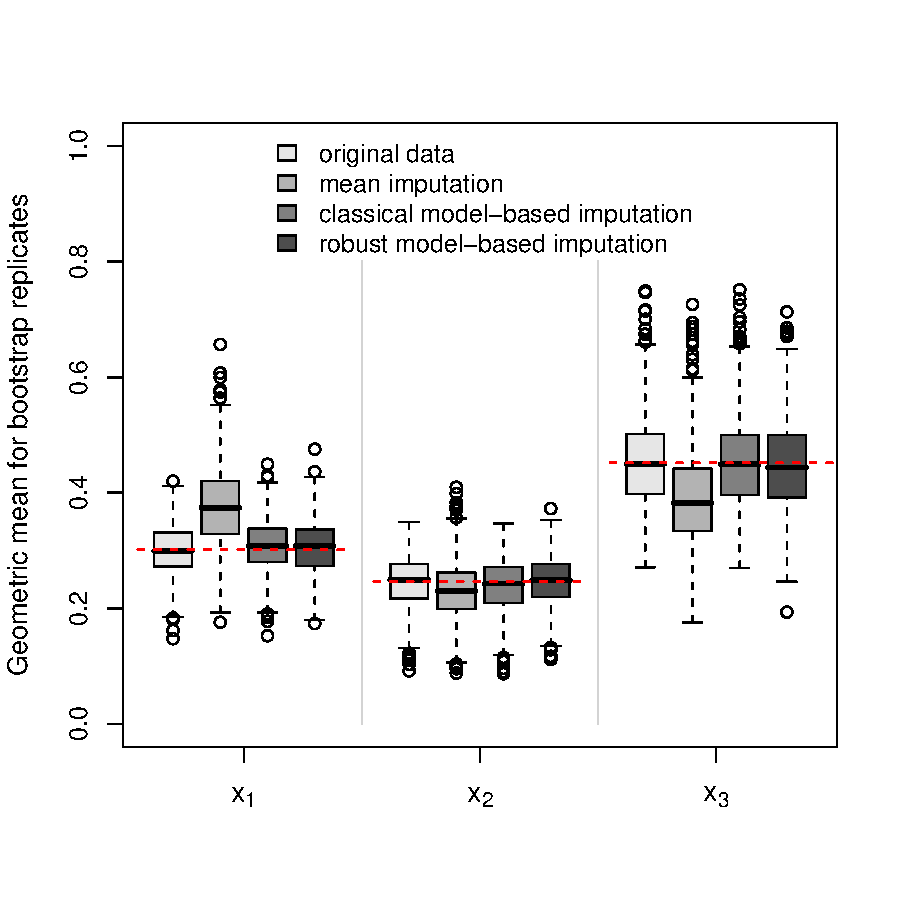
\includegraphics{boxplot}
\vspace*{-1cm}
\caption{\label{boxplot}Boxplot comparison of the estimated column-wise geometric means of
$1000$ bootstrap replicates of the original data set and the data sets 
where missing values were imputated with different methods. The red line
is the column-wise geometric mean of the original data. Outliers are excluded
in the computation of the geometric means.}
\end{center}
\end{figure}

\begin{knitrout}
\definecolor{shadecolor}{rgb}{0.969, 0.969, 0.969}\color{fgcolor}\begin{kframe}
\begin{alltt}
\hlstd{R} \hlkwb{<-} \hlnum{5}
\hlkwd{bootimp}\hlstd{(x}\hlopt{$}\hlstd{z2,} \hlkwc{R}\hlstd{=R)}
\end{alltt}
\end{kframe}
\end{knitrout}


%<<bootstat-erg-lm>>=
%bootimp(x$zmiss, R=R)
%@

%With our generated data set, we see that method ``ltsReg'' includes a little bit more uncertainty:

%<<bootstat-erg-ltsReg>>=
%bootimp(x$zmiss, R=R)
%@

%However, with other choices of the data generation process, method ``ltsReg'' results in closer confidence intervals than method ``lm''.
%Please note, that other imputation methods might include much more uncertainty.


\subsection{Diagnostic Plots}

Here we do not assume knowledge about the observed values. The goal is to visualize
the imputed values in an appropriate way. Because of space limitations we
only show results for the robust model-based procedure.

The first diagnostic plot is a multiple
scatterplot where the imputed values are compared with the observed ones. 
This plot can be generated with 
\begin{knitrout}
\definecolor{shadecolor}{rgb}{0.969, 0.969, 0.969}\color{fgcolor}\begin{kframe}
\begin{alltt}
\hlkwd{plot}\hlstd{(xImp1,} \hlkwc{which}\hlstd{=}\hlnum{1}\hlstd{)}
\end{alltt}
\end{kframe}
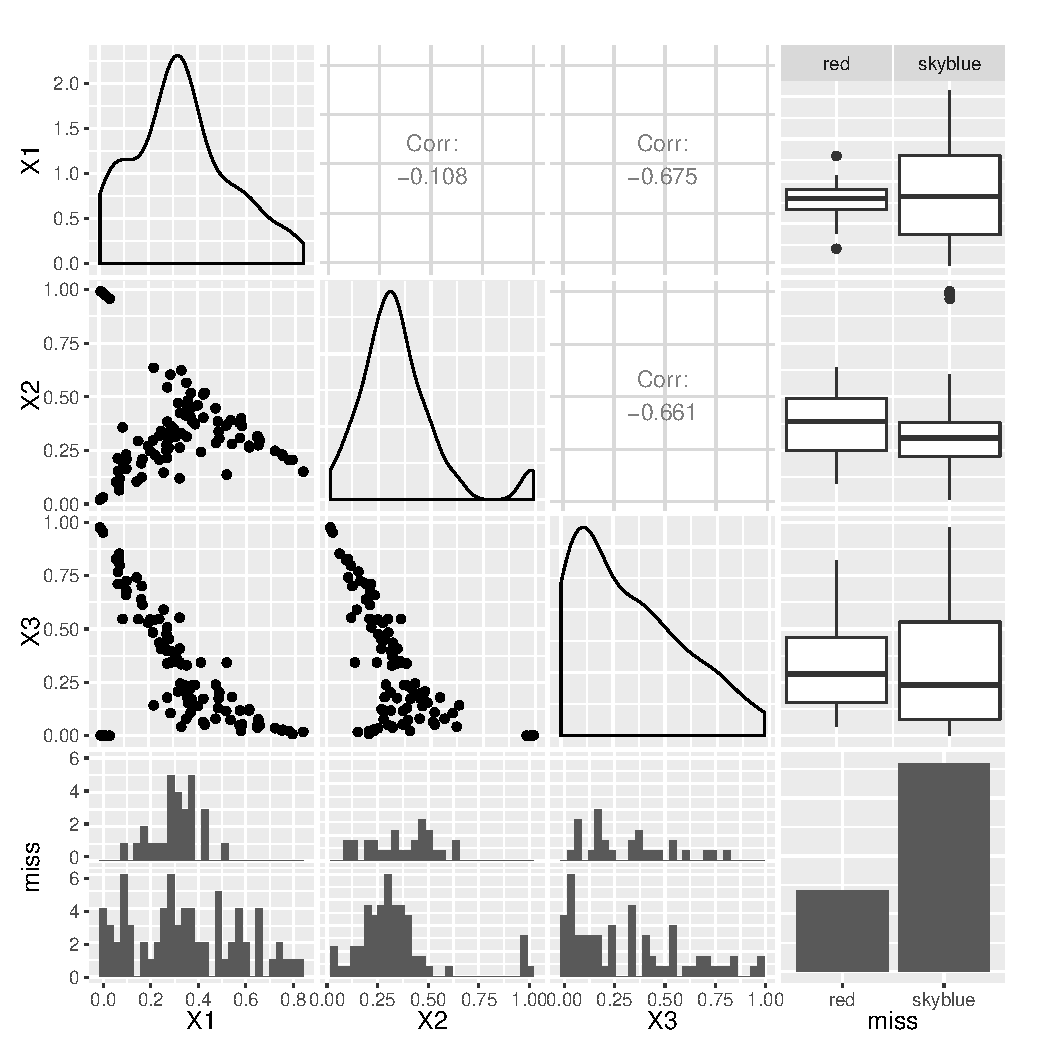
\includegraphics[width=\maxwidth]{figure/unnamed-chunk-4-1} 

\end{knitrout}

To avoid that imputed values are 
placed on the regression hyperplane(s), one
can add random noise to the imputed values. This can be done with the function
\texttt{impCoda()} using the parameter \texttt{method $=$ ltsReg2} which considers
the standard deviation of the residuals for generating the random noise. 
% This plot can also be generated for instance for log-ratio transformed data
% \citep{Aitchison86}, taking care of the compositional nature of the data.
% 

%' %Note that this plot cannot be applied after an isometric log-ratio transformation
%' %because the dimension of the data is reduced by 1.
%' 
%' %\begin{center}
%' %\begin{figure}[h]
%' %<<plot1, fig=TRUE>>=
%' %plot(xImp1, which=1)
%' %@
%' %\caption{Multiple Scatterplot to highlight observation which includes
%' %imputations resulting from $k$-nearest neighbor imputation within the
%' %Aitchison space.}
%' %\label{repFig1}
%' %\end{figure}
%' %\end{center}
%' 
%' \begin{figure}[h]
%' \begin{center}
%' <<plot1,echo=FALSE>>=
%' dimnames(xImp2$xImp)[[2]] <- c("x1","x2","x3")
%' plot(xImp2, which=1)
%' @
%' \vspace*{-0.4cm}
%' \caption{\label{repFig1b}Multiple Scatterplot to highlight imputed observations.}
%' \end{center}
%' \end{figure}

A parallel coordinate plot \citep{Wegman90} can be generated by 

\begin{knitrout}
\definecolor{shadecolor}{rgb}{0.969, 0.969, 0.969}\color{fgcolor}\begin{kframe}
\begin{alltt}
\hlkwd{plot}\hlstd{(xImp1,} \hlkwc{which}\hlstd{=}\hlnum{2}\hlstd{)}
\end{alltt}
\end{kframe}
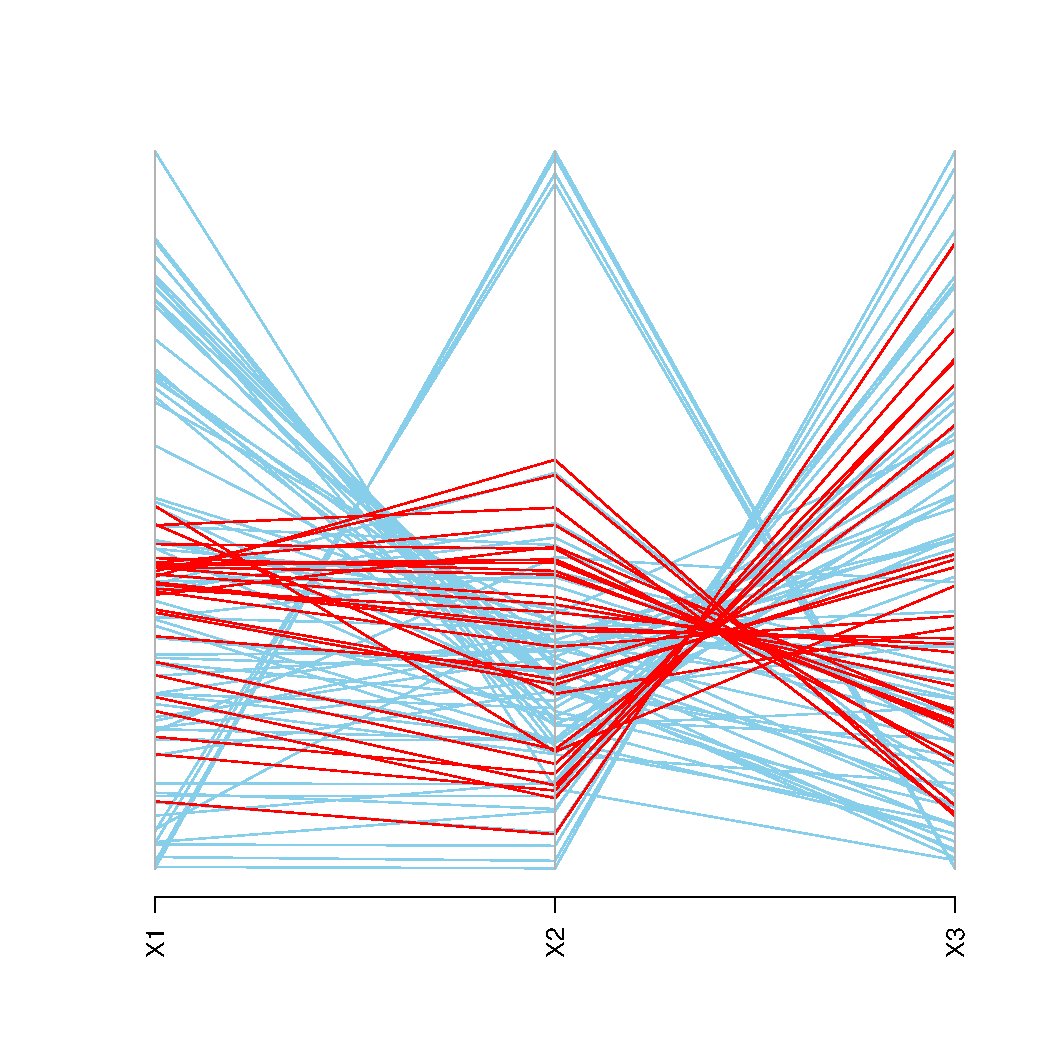
\includegraphics[width=\maxwidth]{figure/unnamed-chunk-5-1} 

\end{knitrout}
%' (plot not shown here). 
The imputed values in certain variables are highlighted.
One can select variables interactively, and imputed values in any of the 
 selected variables will be highlighted. 
%' 
%' %\begin{center}
%' %\begin{figure}[h]
%' %<<plot2, fig=TRUE>>=
%' %plot(xImp2, which=2, interactive = FALSE)
%' %@
%' %\vspace*{-1cm}
%' %\caption{Interactive parallel coordinate plot of object \texttt{xImp2} in which
%' %observations with imputed values are highlighted in \textcolor{red}{red}.}
%' %\label{repFig2}
%' %\end{figure}
%' %\end{center}
%' 


The third diagnostic plot (see Figure \ref{repFig4}), a ternary diagram \citep{Aitchison86},
 can be generated with 
 
\begin{knitrout}
\definecolor{shadecolor}{rgb}{0.969, 0.969, 0.969}\color{fgcolor}\begin{kframe}
\begin{alltt}
\hlkwd{plot}\hlstd{(xImp1,} \hlkwc{which}\hlstd{=}\hlnum{3}\hlstd{,} \hlkwc{seg1}\hlstd{=}\hlnum{FALSE}\hlstd{)}
\end{alltt}
\end{kframe}
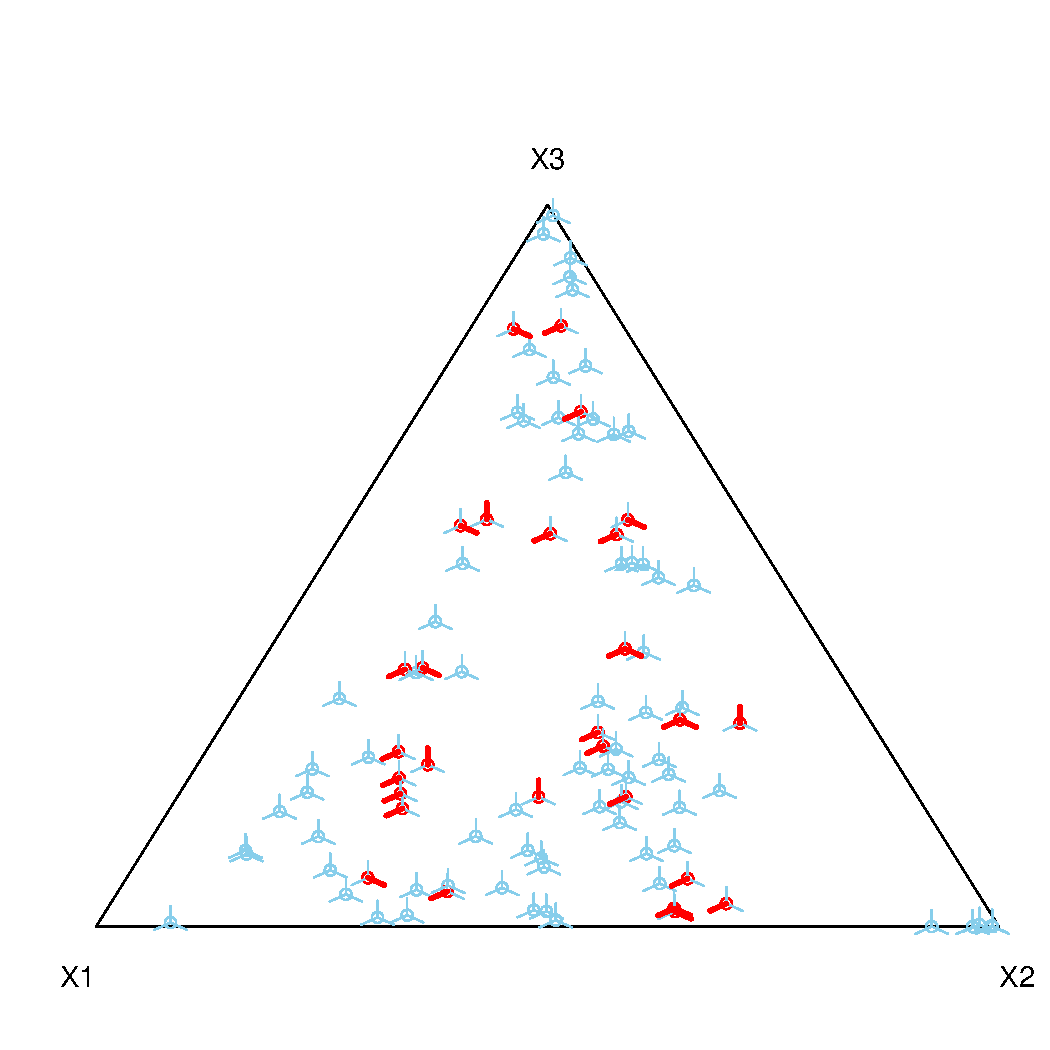
\includegraphics[width=\maxwidth]{figure/unnamed-chunk-6-1} 

\end{knitrout}

The 3-part compositions are presented by three spikes, pointing in the
 directions of the corresponding three variables. The spikes of
 the imputed values are highlighted. This presentation allows gaining a multivariate
 view of the data, being helpful for interpreting possible irregularities
 of imputed values.

%' %\begin{center}
%' %\begin{figure}
%' %<<plot4, fig=TRUE>>=
%' %plot(xImp1, which=3, seg1=FALSE)
%' %@
%' %\caption{ternary plot with plotting symbols with no justification.}
%' %\label{repFig4}
%' %\end{figure}
%' %\end{center}
%' 
%' \setkeys{Gin}{width=0.6\textwidth}
%' \begin{figure}[h]
%' \begin{center}
%' <<plot4, echo=FALSE>>=
%' par(mar=c(0,0,0,0))
%' dimnames(xImp2$xImp)[[2]] <- c("x1","x2","x3")
%' plot(xImp2, which=3, seg1=FALSE)
%' @
%' \vspace*{-3mm}
%' \caption{\label{repFig4}Ternary diagram with special plotting symbols for highlighting imputed
%' parts of the compositional data.}
%' \end{center}
%' \end{figure}
%' 
%' 

\section{Conclusions}

We provide the R-package \texttt{robCompositions} which includes advanced methods for 
imputation for compositional data. We have shown how the imputation
methods described in \cite{Hron09} can be applied with the package.
The methods are especially designed for data including outliers.
The performance of the methods is outlined in the original paper.

The package includes possibilities for evaluating the quality of
the imputed values: One can compute measures for information loss,
use bootstrapping for estimating bias and uncertainty of parameters,
and visualize the imputed values with diagnostic tools.
For 3-dimensional compositions the proposed ternary plot is designed 
to highlight how well imputations are made and which compositions were imputed.
Note that many additional options
can be used within these plots given by the arguments of the 
plotting function.
%' 
%' %\newpage

%\footnotesize
\bibliography{refPCS}{}
\bibliographystyle{plainnat}

\end{document}
